
%%%%%%%%%%%%%%%%
%              %
% Title page   %
%              %
\pagestyle{empty}
\tikz[remember picture,overlay] \node[inner sep=0pt] at (current page.center){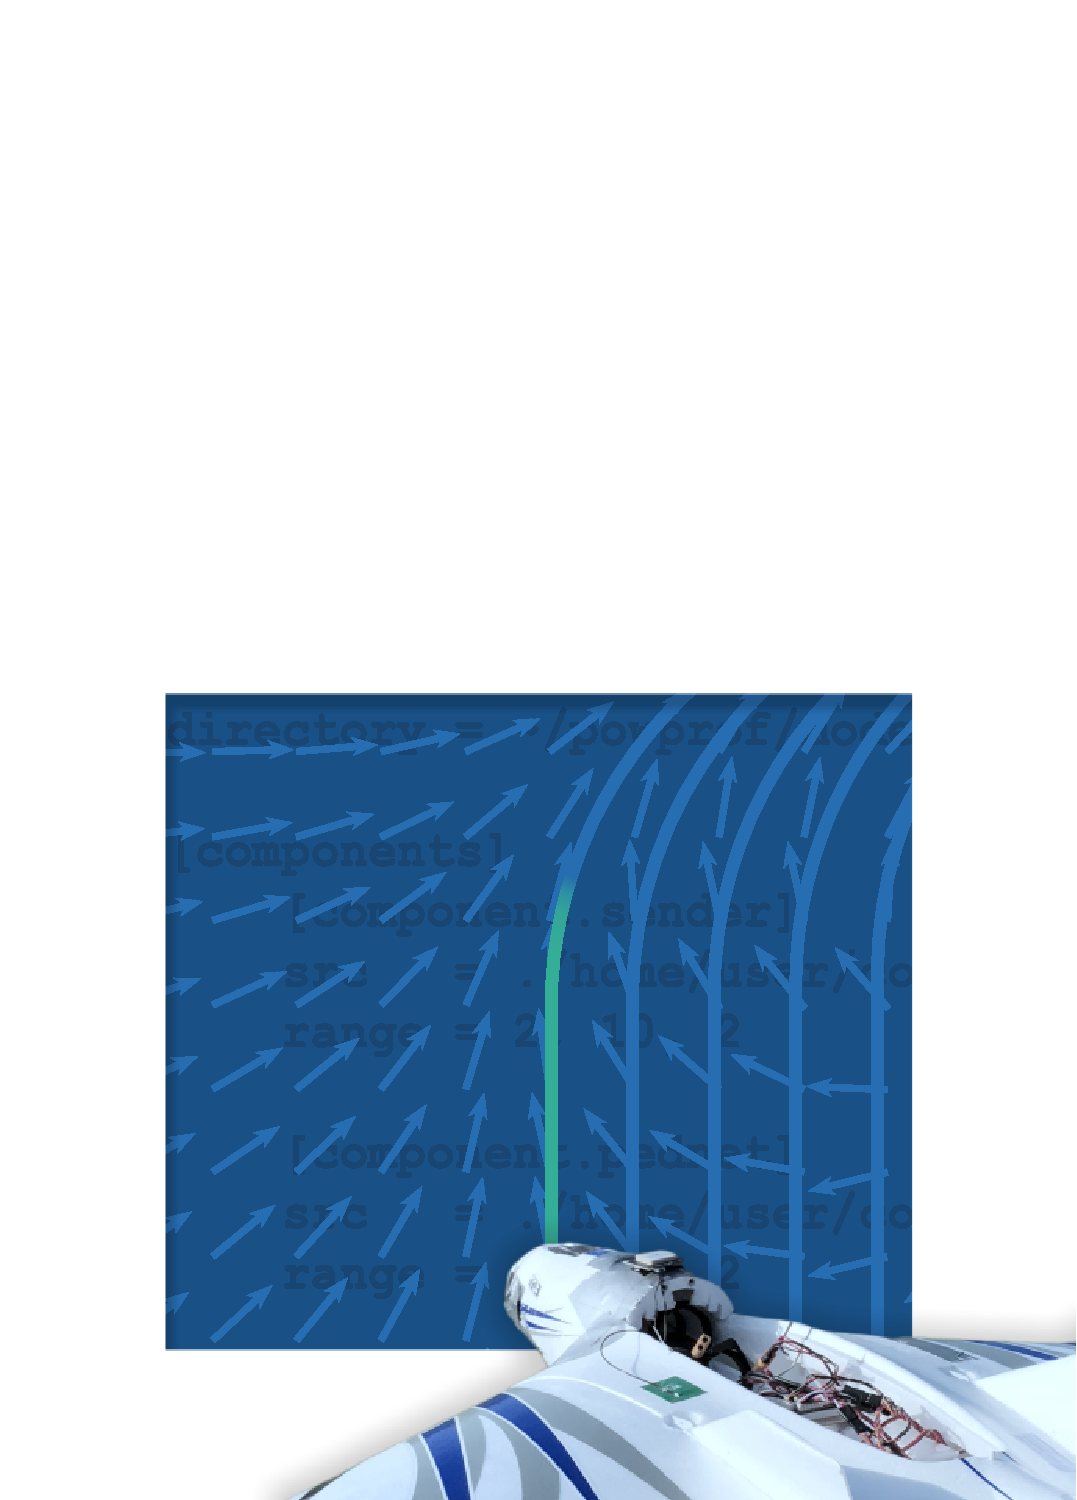
\includegraphics[width=\paperwidth,height=\paperheight]{figures/source/cover3.pdf}};
{
\centering
	{\large ~\par}
	~

	\vspace{28pt}
	{\Huge\fontfamily{phv}\selectfont\bfseries\booktitle\par}
	\vspace{24pt}

	{\Large\fontfamily{phv}\selectfont\authorname\par}

}
\cleardoublepage

%\pagestyle{empty}
%\tikz[remember picture,overlay] \node[inner sep=0pt] at (current page.center){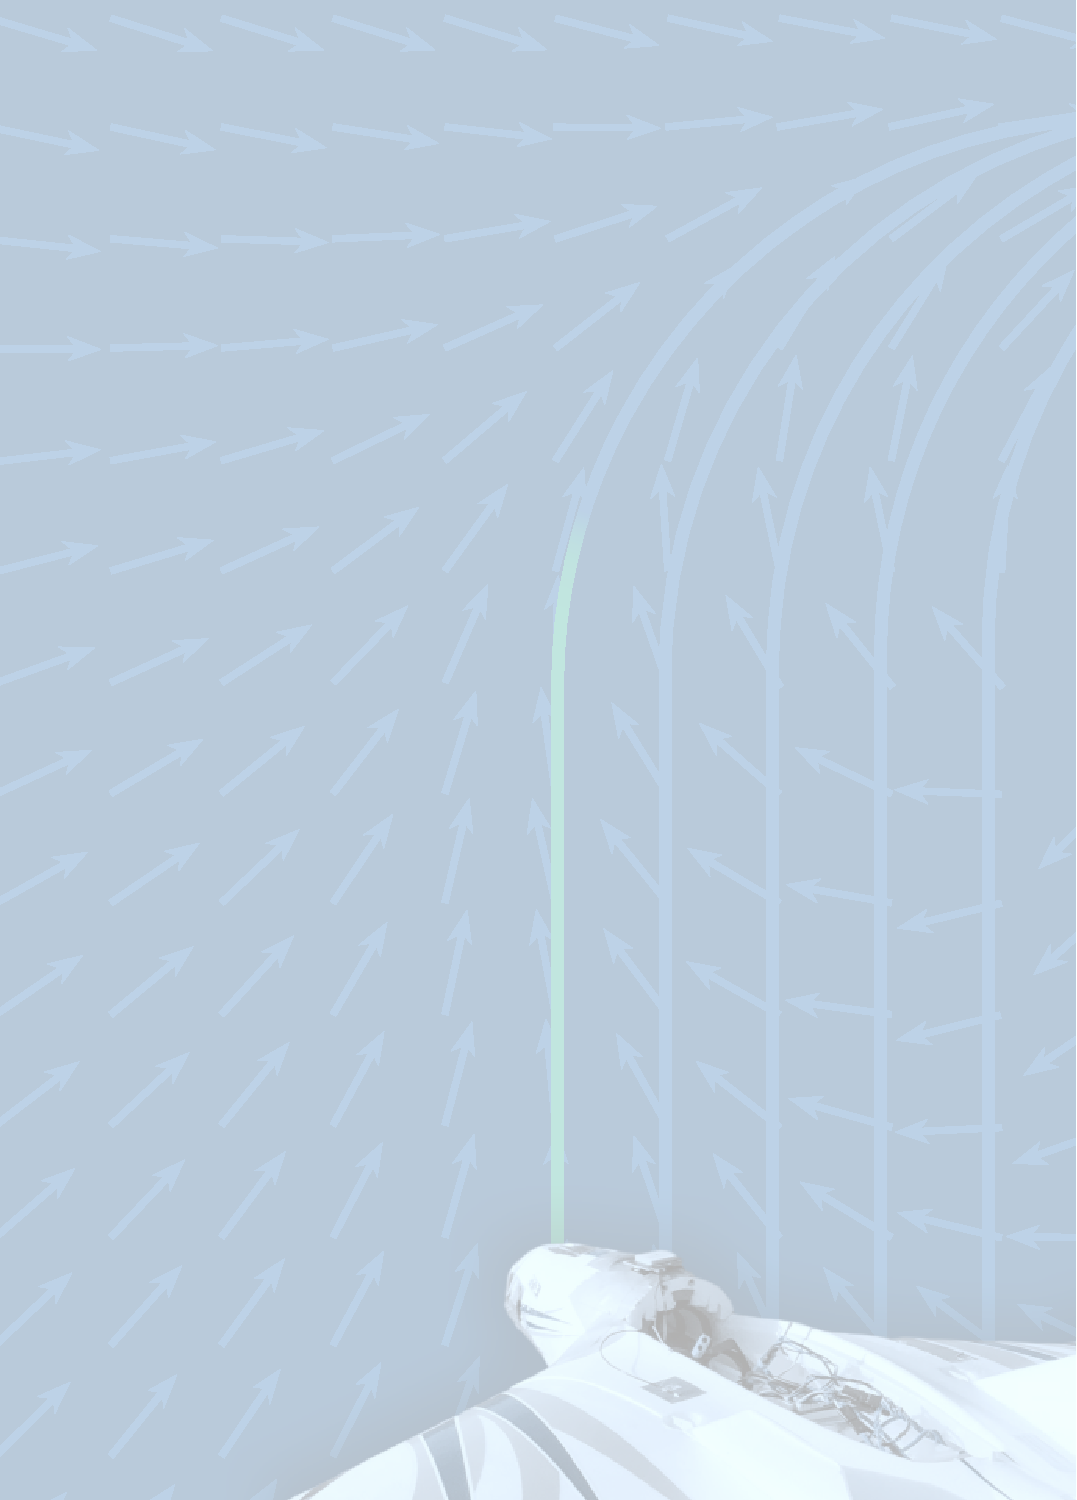
\includegraphics[width=\paperwidth,height=\paperheight]{figures/source/cover2.pdf}};
%{
%\centering
%	~
%}
%\cleardoublepage


\begin{titlepage}
	\centering
	{\large \publisher\par}
	~

	\vspace{28pt}
	{\Huge\fontfamily{phv}\selectfont\bfseries\booktitle\par}
	\vspace{24pt}

	{\Large\fontfamily{phv}\selectfont\authorname\par}
	\vspace{24pt}

	\vspace{\stretch{1.25}}
	{\large A dissertation submitted in partial satisfaction of the\par\vspace*{.8ex}
	requirements for the degree Doctor of Philosophy\par\vspace*{.8ex}
	in Engineering Science}
	\vspace{42pt}

	{\begin{flushleft}%{\itshape Committee in charge:}
		\begin{multicols}{2}
			%{Ulrik Pagh Schultz, Advisor\\\vspace*{.8ex}
			%Letizia Marchegiani, Member\\\vspace*{.8ex}
			%~, Member\\\vspace*{.8ex}
			%~, Chair\\
			%}\par
			\columnbreak
			{~\\
			~\\
			~}\par
		\end{multicols}
		\vspace{6pt}
		\begin{multicols}{2}
		~\\\columnbreak %{\itshape Approved on:}
		\end{multicols}	
	\end{flushleft}}

	\vspace{\stretch{6}}
	{\large\centering\editionyear{}}
\end{titlepage}

